\section{Partial Derivatives}

\begin{definition}[Partial derivative]
Given a function $f(x,y)$, we want to define a derivative for $f(x,y)$. Since we have two variables, we can define the derivative using only one of them. Recall that for functions of one variable:
$$
f'(a) = \lim_{h\to 0}{\frac{f(a+h)-f(a)}{h}} \qquad \text{provided that the limti exists.}
$$
If we fix the value of $y$ and we use values $(x,y)$ to approach $(a,b)$, we define the partial derivative of $f(x,y)$ with respect to $x$ as
$$
\partialderiv{}{x} f(x,y) = \lim_{h\to0}\frac{f(x+h,y)-f(x,y)}{h}
$$
Similarly, if $x$ is fixed, the partial derivative with respect to $y$ can be defined as
$$
\partialderiv{}{y} f(x,y) = \lim_{h\to0}\frac{f(x,y+h)-f(x,y)}{h}
$$
provided that the limits exist.
\end{definition}

There are different ways to denote the partial derivative
$$
f_x =   f_x(x,y) = \partialderiv{f}{x} = \partialderiv{}{x}f(x,y)
$$

\section{Tangent Plane}

\subsection{Definition}
Given $f(x,y)$ and point $(a,b,c)$ on the surface, the plane tangent to the surface at $(a,b,c)$ is
$$
z-c = f_x(a,b)(x-a) + f_y(a,b)(y-b)
$$

\subsection{Linear Approximation}
Differentiable functions are locally linear, meaning that if zoom in close enough, the function will appear to be linear. Because of that, we can approximate the value of the function near $(a,b)$ using the tangent plane at that point.

Let $L$ be the linear function that is the tangent plane at point $(a,b)$.
$$
L(x,y) = f(a,b) + f_x(a,b)(x-a) + f_y(a,b)(y-b)
$$
$L$ is called the linearization of $f$ at $(a,b)$, and we can use that to approximate the value of $f$ at points near $(a,b)$.
$$
f(x,y) \approx f(a,b) + f_x(a,b)(x-a) + f_y(a,b)(y-b)
$$

\section{Higher Order Derivatives}

\begin{theorem}[Clairaut's Theorem (symmetry of second derivatives)]
Suppose that $S \subseteq \R^n$ is open. If $f\; S \to \R$ is twice continuously differentiable (of class $C^2$), then
$$
\frac{\partial^2 f}{\partial x_i \partial x_j} = 
\frac{\partial^2 f}{\partial x_j \partial x_i}
$$
for all $i,j=1,\cdots, n$ everywhere in $S$.
\end{theorem}

The proof of the Clairaut's Theorem utilizes the Mean Value Theorem.

We can expand the Clairaut's Theorem to higher-order derivatives.

\begin{theorem}
Suppose that $S$ is an open subset of $\R^n$ and that $f:\;S \to \R$ is of class $C^k$. For any integers $i_1,\cdots,i_k$ between $1$ and $n$, if $j_1,\cdots,j_k$ is a reordering of $i_1,\cdots,i_k$, then
$$
\frac{\partial}{\partial x_{i_k} }\cdots 
\frac{\partial}{\partial x_{i_1} }f
\ = \ 
\frac{\partial}{\partial x_{j_k} }\cdots 
\frac{\partial}{\partial x_{j_1} }f
$$
everywhere in $S$.
\end{theorem}
This theorem can be proved from the Clairaut's Theorem using induction.

\section{The Chain Rule}

\subsection{Review: Chain rule for single-variable functions}
For $f(x)$ where $x=g(t)$
$$
\frac{df}{dt} = \frac{df}{dx}\frac{dx}{dt}
$$
or equivalently
$$
\frac{df}{dt} = f'(g(t)) \cdot g'(t)
$$

\subsection{Multivariable Chain Rule}

\begin{theorem}[The Chain Rule - 1]
If $f(x,y)$ is a function and $x=g(t)$ and $y=h(t)$, then
$$
\frac{df}{dt} = \partialderiv{f(x,y)}{x} \frac{dx}{dt} + \partialderiv{f(x,y)}{y} \frac{dy}{dt}
$$
\end{theorem}

\begin{theorem}[The Chain Rule - 2]
Suppose that $z=f(x,y)$ is a differentiable function of $x$ and $y$, where $x = g(s,t)$ and $y=h(s,t)$ are differentiable functions of $s$ and $t$. Then
$$
\partialderiv{z}{s} = \partialderiv{z}{x}\partialderiv{x}{s} + \partialderiv{z}{y}\partialderiv{y}{s} \qquad \partialderiv{z}{t} = \partialderiv{z}{x}\partialderiv{x}{t} + \partialderiv{z}{y}\partialderiv{y}{t}
$$
\end{theorem}

\begin{center}
    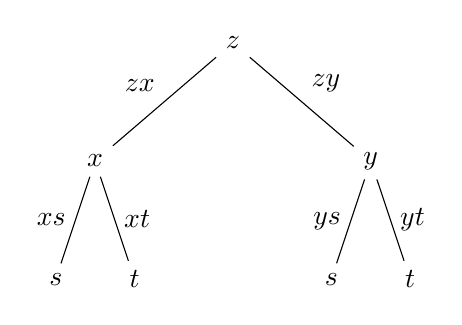
\begin{tikzpicture}[level distance=1.5cm,
    level 1/.style={sibling distance=3.5cm},
    level 2/.style={sibling distance=1cm}]
    \node {$z$}
        child {  
            node {$x$}
            child {
                node {$s$}
                edge from parent node[left,draw=none] {$\partialderiv{x}{s}$}
            }
            child {
                node {$t$}
                edge from parent node[right,draw=none] {$\partialderiv{x}{t}$}
            }
            edge from parent node[above left,draw=none] {$\partialderiv{z}{x}$}
        }
        child {  
            node {$y$}
            child {
                node {$s$}
                edge from parent node[left,draw=none] {$\partialderiv{y}{s}$}
            }
            child {
                node {$t$}
                edge from parent node[right,draw=none] {$\partialderiv{y}{t}$}
            }
            edge from parent node[above right,draw=none] {$\partialderiv{z}{y}$}
        };
    \end{tikzpicture}
\end{center}

\begin{theorem}[The Chain Rule - General Case]
Suppose that $u$ is a differentiable function of the $n$ variables $x_1, x_2, \cdots , x_n$ and each $x_j$ is a differentiable function of the $m$ variables $t_1, t_2, \cdots , t_m$. Then $u$ is a function of $t_1, t_2, \cdots, t_m$ and
$$
\partialderiv{u}{t_i} = \partialderiv{u}{x_1}\partialderiv{x_1}{t_i} + \cdots + \partialderiv{u}{x_n}\partialderiv{x_n}{t_i} = \sum_{j=1}^n \partialderiv{u}{x_j}\partialderiv{x_j}{t_i}
$$
\end{theorem}

\subsection{Generalization}
We can further generalize the Chain Rule using Jacobian matrix and matrix multiplication.

If $\mathbf g$ is differentiable at $\mathbf a$, and $\mathbf f$ is differentiable at $\mathbf{g}(\mathbf{a})$, then the composite function $\mathbf f \circ \mathbf g$ is differentiable at $\mathbf a$ and
$$
D(\mathbf f\circ\mathbf g)(\mathbf a) = [D\mathbf f(\mathbf g(\mathbf a))] \ [D\mathbf g(\mathbf a)].
$$
where $D\mathbf f$ denotes the Jacobian of $\mathbf f$
$$
D\mathbf f = \left[ \partialderiv{\mathbf f}{x_1}, \cdots, \partialderiv{\mathbf f}{x_2} \right]
$$
Writing this as individual components and partial derivatives gives
$$
\frac {\partial }{\partial x_j} (f_k\circ \mathbf g)(\mathbf a) 
=\sum_{i=1}^m \frac{\partial f_k}{\partial y_i}(\mathbf g(\mathbf a)) \ \frac{\partial g_i}{\partial x_j}(\mathbf a)
$$

\section{Differentiability}

\subsection{Definitions}

\begin{definition}[Differentiability for single variable]
If $z=f(x)$, then $f$ is differentiable at $x$ if there exists $m$ and $\epsilon$ such that $\Delta z$ can be expressed in the form
$$
\Delta z = f(x+h)-f(x) = mh + \epsilon h \qquad \text{ and } \qquad \lim_{h \to 0} \frac{\epsilon h}{h} = \lim_{h\to 0} \epsilon = 0
$$
The value of $m$ is the derivative of $f$ evaluated at $x$ (i.e. $f'(x)=m$).
\end{definition}

This equivalent definition can be understood as follows: temporarily fix $x$, treat $h$  as a variable, and view $\Delta z = f(x+h)-f(x)$ as a function of $h$. Then $f$ is differentiable at $h$ if $\Delta z$ is approximately $mh$, with an error term $\epsilon h$ that approaches zero as $h \to 0$.

In other words, this definition says that a function is differentiable if the linear approximation of the function is a good approximation at $x$ when for values close to $x$.

\begin{figure}[h]
    \centering
    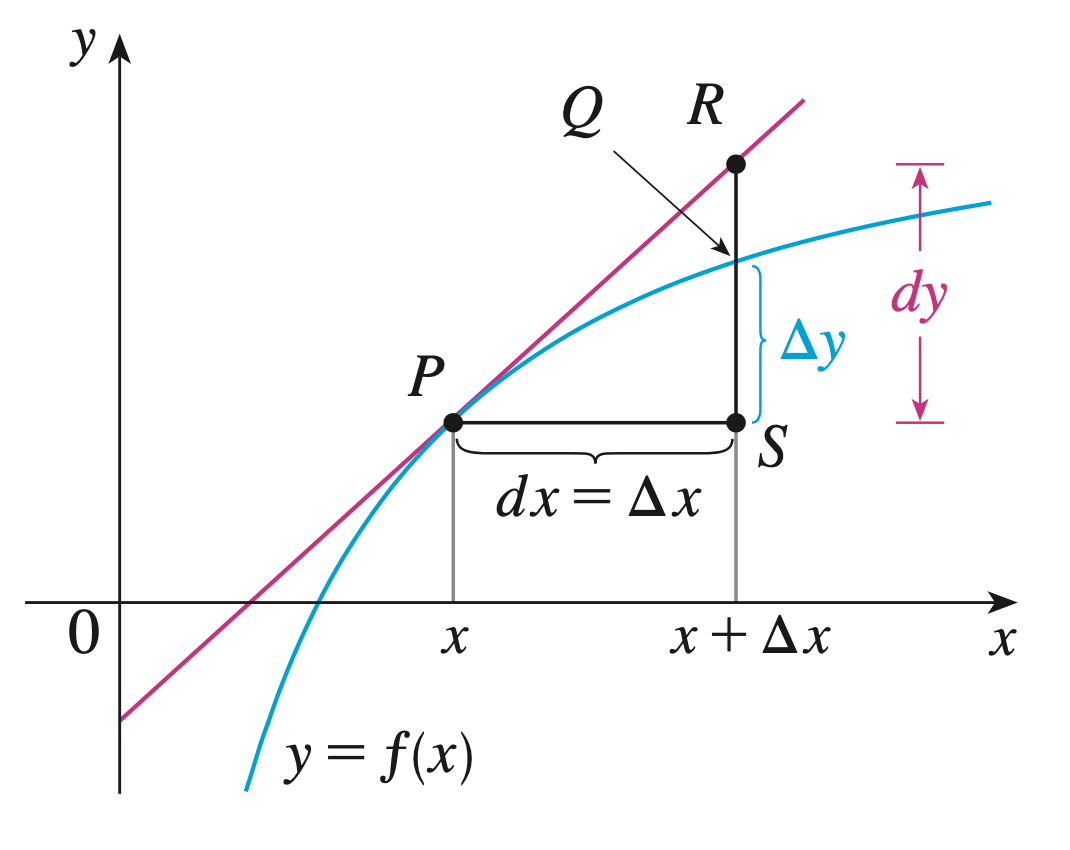
\includegraphics[width=0.4\linewidth]{figures/linear-appox.png}
    \caption{Linear approximation}
    \label{fig:linear-approx}
\end{figure}

We can extend this definition to functions with multiple variables.

\begin{definition}[Differentiability for multiple variables]
If $z=f(x,y)$, then $f$ is differentiable at $(x,y)$ if there exists $m,n$ and $\epsilon_1, \epsilon_2$ such that $\Delta z$ can be expressed in the form
$$
\Delta z = m \Delta z + n \Delta y + E_1(\Delta x) + E_2(\Delta y)
$$
and $\epsilon_1 \to 0, \epsilon_2 \to 0$ as $(\Delta x, \Delta y) \to (0,0)$. $m=f_x(x,y)$ and $n=f_y(x,y)$.
\end{definition}

Alternatively, this can be phrased using vectors.
\begin{definition}
Suppose that $f$ is a function. We say that $f$ is differentiable at $x \in \R^n$ if there exists a vector $\vv m \in \R^n$ such that
$$
f(\vv x + \vv h) - f(\vv x) = \vv m \cdot \vv h + E(\vv h)
$$
where $\displaystyle \lim_{\vv h \to 0} \frac{E(\vv h)}{\norm{\vv h}} = 0$.

When this holds, we define $\nabla f(\vv x) = \vv m$
\end{definition}

\subsubsection{Partial Differentiability}

\begin{theorem}[Differentiability implies partial differentiability]
Let $f$ be a function. If $f$ is differentiable at a point $\vv x \in \R^n$, then $\partialderiv{f}{x_j}$ exists for all $j = 1,\cdots, n$, and in addition,
$$
\nabla f(\vv x) = \left(\partialderiv{f}{x_1},\cdots,\partialderiv{f}{x_n}\right)(\vv x)
$$
The converse is NOT true.
\end{theorem}

This theorem can be helpful when determining the differentiability of a function:
\begin{itemize}
    \item If any partial derivative does not exist, then $f$ is not differentiable
    \item If all partial derivative exist, then $\vv m = (\partialderiv{f}{x_1},\cdots,\partialderiv{f}{x_n})$ is the only possible vector that may work in the definition of differentiability.
\end{itemize}

\section{Directional Derivative and Gradient}

\subsection{Directional Derivative}

The directional derivative of $f$ at $(x_0,y_0)$ in the direction of a unit vector $\vv u = (a,b)$ is
$$
\partial_u f(x_0,y_0) = \lim_{h \to 0} \frac{f(x_0+ha, y_0+hb) - f(x_0,y_0)}{h}
$$
provided that the limit exists.

More generally,
$$
\partial_u f(\vv x) = \lim_{h\to 0} \frac{f(\vv x + h\vv u) - f(\vv x)}{h}
$$

\begin{theorem}
If $f$ is differentiable at a point $\vv x$, then $\partial_u f(\vv x)$ exists for every unit vector $\vv u$, and moreover,
$$
\partial_u f(\vv x) = \vv u \cdot \nabla f(\vv x) = \sum_{j=1}^n \partialderiv{f}{x_j}u_j
$$
\end{theorem}

The directional derivative tells us the instantaneous rate of change of the surface at point $\vv x$ in the direction of the unit vector $\vv u$.

\begin{figure}[h]
    \centering
    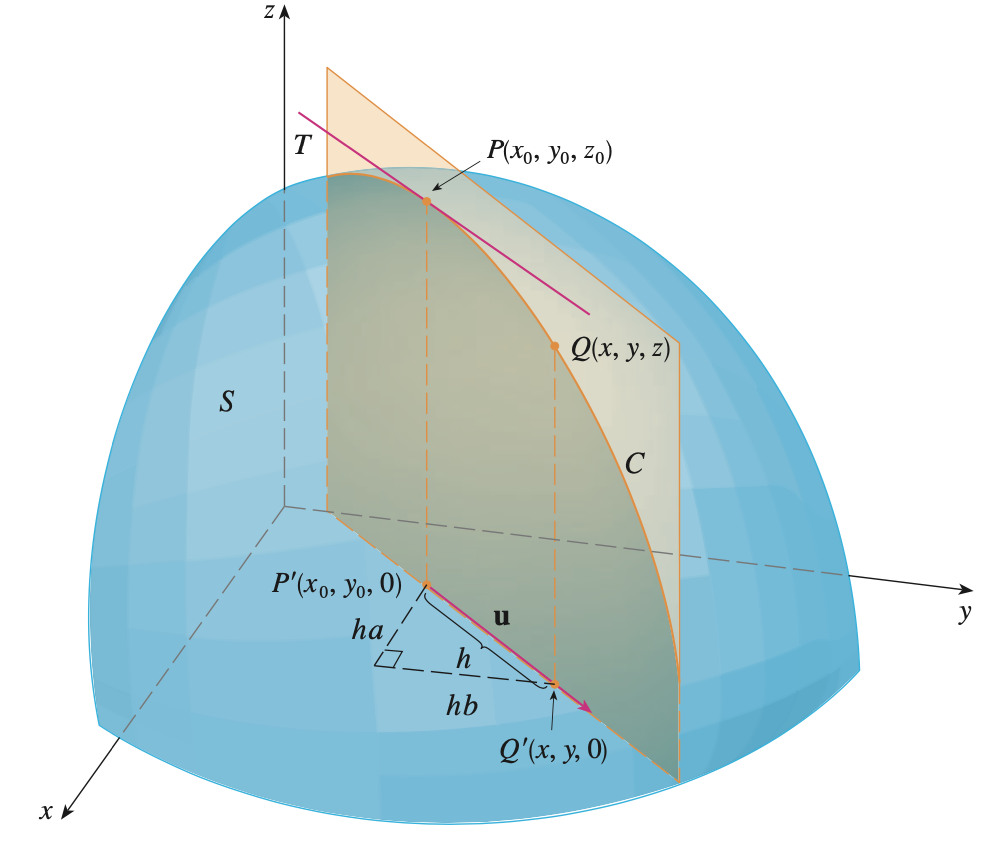
\includegraphics[width=0.5\linewidth]{figures/direcitonal-derivative.png}
    \caption{Directional derivative at $\protect P$ is the slope of the tangent line $\protect T$ to $\protect C$. $\protect C$ is the curve obtained by intersecting the surface with a plane in the direction of $\protect \vv u$}
    \label{fig:directional-derivative}
\end{figure}

In particular, we can see that the partial derivative can be written in terms of directional derivatives. For any $j \in \{1,\cdots,n \}$
$$
\partialderiv{f}{x_j} = \partial_{\hat{e_j}}f
$$
where $\hat{e_j}$ denotes the unit vector in the $j$-th coordinate direction.

\subsection{Gradient}

We defined gradient in the definition of differentiability. We now formally define gradient in terms of partial derivatives.

\begin{definition}[Gradient]
If $f$ is a function, then the gradient of $f$ is the vector function $\nabla f$ defined by
$$
\nabla f(x,y) = \partialderiv{f}{x}\vv i + \partialderiv{f}{y}\vv j
$$
More generally,
$$
\nabla f(\vv x) = \left(\partialderiv{f}{x_i},\cdots,\partialderiv{f}{x_n}\right) (\vv x)
$$
\end{definition}

\begin{theorem}
If it is not zero, $\nabla f(\vv x)$ points in the direction where $f$ has the greatest increase.

\begin{proof}
Since
$$
\partial_u f = \nabla f \cdot \vv u = \norm{\nabla f}\norm{\vv u}\cos\theta = \norm{\nabla f}\cos\theta
$$
The maximum value of $\cos\theta$ is $1$, which occurs when $\theta = 0$. Therefore, the maximum value $\partial_u f$ is $\norm{\nabla f}$ and it occurs when $\theta = 0$, that is when $\vv u$ has the same direction as $\nabla f$.
\end{proof}
\end{theorem}

\section{Maximum and Minimum Values}

\begin{definition}[Critical points]
If $S$ is an open subset of $\R^n$ and $f:\, S \to \R$ is differentiable, then a point $a \in S$ is a critical point if $\nabla f(a)=\vv 0$.
\end{definition}

\subsection{First derivative test}

\begin{theorem}[First derivative test]
If $f$ is differentiable, then every local extremum is a critical point.
\end{theorem}

\subsection{Second derivative test}

\begin{theorem}[Second derivative test]
Suppose the second partial derivatives of $f$ are continuous on a disk with center $(a,b)$, and suppose that $f_x(a,b)=0$ and $f_y(a,b)=0$. Let,
$$
D= D(a,b) = f_{xx}(a,b) f_{yy}(a,b) - [f_{xy}(a,b)]^2
$$
Then
\begin{itemize}
    \item If $D>0$ and $f_{xx}(a,b) > 0$, then $f(a,b)$ is a local minimum
    \item If $D>0$ and $f_{xx}(a,b) < 0$, then $f(a,b)$ is a local maximum
    \item If $D<0$ then $(a,b)$ is a saddle point of $f$
    \item If $D=0$, the test is inconclusive
\end{itemize}
\end{theorem}

\subsection{A More Technical Formulation of the Second Derivative Test}

\subsubsection{Hessian Matrix}
\begin{definition}[Hessian matrix]
$$
H = Hf= \left(\begin{array}{ccc}
\partial_1\partial_1 f & \cdots & \partial_1\partial_n f \\
\vdots & \ddots & \vdots \\
\partial_n\partial_1 f & \cdots & \partial_n\partial_n f 
\end{array}
\right)
$$
For example, for functions of two variables, the Hessian matrix is defined as
$$
H = Hf= \left(\begin{array}{ccc}
\partial_x\partial_x f & \partial_x\partial_y f \\
\partial_y\partial_x f & \partial_y\partial_y f
\end{array}
\right) =
\left(\begin{array}{ccc}
f_{xx} & f_{xy} \\
f_{yx} & f_{yy}
\end{array}
\right)
$$
\end{definition}

\subsubsection{Properties of Symmetric Matrices}

Given a symmetric $n\times n$ matrix with entries $a_{ij}$ for $i,j \in \{1,\cdots, n\}$, we can define a function $\R^n \to \R$
$$
\vv x \mapsto (A\vv x)\cdot \vv x = \sum_{i,j=1}^n a_{ij}x_ix_j
$$

\begin{definition}[Definite matrices]
A symmetric $n\times n$ matrix is
\begin{itemize}
    \item positive definite if $\vv x^\top A \vv x > 0$ for all $\vv x \neq 0$
    \item nonnegative definite if $\vv x^\top A \vv x \geq 0$ for all $\vv x \in \R^n$
\end{itemize}
In addition, we say that $A$ is
\begin{itemize}
    \item negative definite if $-A$ is positive definite
    \item nonpositive definite if $-A$ is nonnegative definite
\end{itemize}
Otherwise if none of the above holds, the we say that $A$ is indefinite. Equivalently, $A$ is indefinite if
$$
\exists \vv x, \vv y \in \R^n,\; \vv x^\top A \vv x < 0 < \vv y^\top A \vv y
$$
\end{definition}